% 电生理结果
% - [ ] 能量谱提示主要的波段
% - [ ] 能量曲线的变化
% - [ ] 相位分析显示学习过程

\section{电生理记录与脑电频谱变化}
由于临床需要,医用不锈钢电极被放置在每位患者主要癫痫病灶区域,
用以监测和定位癫痫的起始位置。通过与华山医院的合作,以及患者
的同意,我们得以在患者进行行为学测试的同时,记录下相应电极的
电信号。癫痫多发与颞叶,而电极的主要记录位置因而集中在颞叶;
但其中有一例特别的病例,患者\#1的癫痫病灶集中在枕叶,因而得以
记录到来自视觉皮层的脑电信号(图\ref{fig:ephys_example}~a)。

\subsection{能量谱提示主要的波段}
我们首先对原始的数字信号进行了小波变化处理,将每次光栅刺激的脑电信号
依据光栅开始的时间对齐,做出脑电信号频谱图(图\ref{fig:ephys_example}~c)。
通过频谱图可见,患者脑电的主要频谱集中在50至100赫兹,即\(\gamma\)波段(\(30 \sim 80 \text{Hz}\))。
这与过去脑电记录相关的实验结果相符合\cite{todo}。%TODO

为了进一步量化脑电信号能量的变化,我们依据频谱获得的频率范围以及\(\gamma\)波段范围,选取了
相对应的50至80赫兹作为后续的探究范围。我们计算得到经过带通滤波的脑电信号的能量变化,
并经过z-score归一化得到每个通道的能量曲线(图\ref{fig:ehpys_example}~d)。
与能量频谱相同,能量曲线在光栅开始后也出现了明显的增强,并横跨了整个刺激期间。

我们对小鼠的局部场电位信号也做了相同的分析处理(图\ref{fig:ephys_example}~f, g),
可以看到小鼠的频谱与患者的频谱相似,同样也涵盖了\(\gamma\)波段;
但相较而言小鼠的总体振荡比患者的稍偏低频一些。
而小鼠的能量曲线也同样在光栅开始后出现了明显的增强,并横跨了整个刺激期间。

\begin{figure}[h]
    \centering
    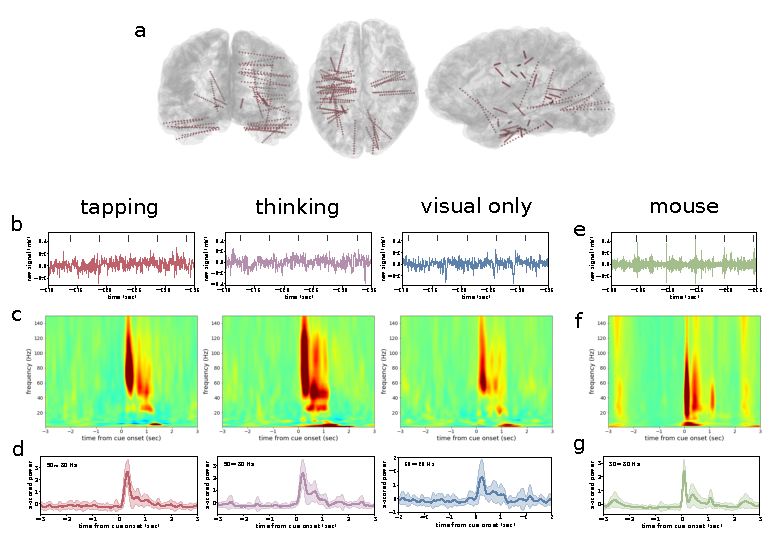
\includegraphics[width=\textwidth]{src/figures/ephys_examples.pdf}
    \caption{\textbf{电生理记录通道示例}\\
    (\textbf{a})~电极的脑区定位。}
    \label{fig:ephys_example}
\end{figure}

\subsection{能量曲线的变化趋势}
依据患者的术前MRI和术后CT,我们得以对每个电极进行定位。
我们从患者\#1中选择了通道数目最多的三个脑区,
视觉皮层(visual cortex, 主要为Brodmann分区17、18、19),
扣带回(cingulate cortex, 主要为Brodmann分区22), %TODO
以及颞中回(middle temporal gyrus, 主要为Brodmann分区)。%TODO

对相同脑区下的脑电能量曲线进行平均后(图\ref{fig:ehpys_network}~a),
我们发现三个脑区的能量曲线形态十分相似,提示光栅刺激可能会引起全脑范围的活动。
%TODO: 视觉的处理
另一方面,对于三种不同的行为范式,轻拍手和默想下的能量曲线基本一直,而空想下的
能量曲线较前两者

\subsection{相位分析显示学习过程}

\begin{figure}[h]
    \centering
    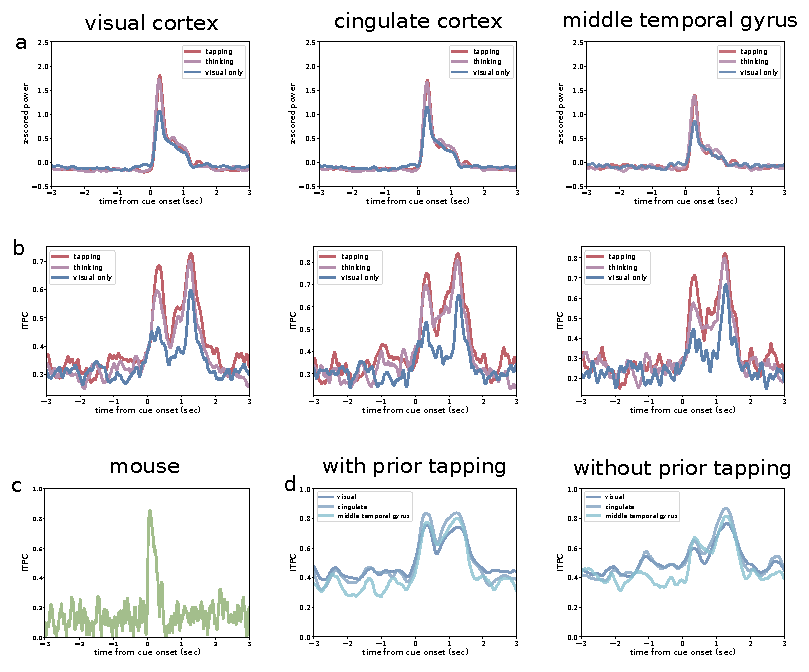
\includegraphics[width=\textwidth]{src/figures/ephys_network.pdf}
    \caption{\textbf{相位分析}\\
    (\textbf{a})~电极的脑区定位。}
    \label{fig:ephys_network}
\end{figure}

